\section{Bootstrap Sampling Reddit Comments for Analysis}
Having established the process for identifying macro norm violating comments on Reddit, we proceeded to apply this process to study the prevalence and characteristics of such comments. Our core strategy for doing this was to take random samples of the online comments from our study subreddits, calculating the classifier agreement scores for each of the samples’ elements, and then taking random samples from those comments that were flagged as potentially norm violating (classifier agreement $\geq 80$). But this effectively meant that we were sampling from different subsets of the population in which some of our random samples have a lower rate of violating comments than others due to the differences in the rate of violating comments between different subreddits. 

This makes drawing conclusions from our samples using the traditional inferential statistics problematic---we cannot simply calculate a binomial proportion confidence interval, because we have several convolved sources of uncertainty. The most straightforward parametric statistical procedure would be to select random comments, label them as violating or not violating, and estimate overall levels of violation from that. Unfortunately, due to the large class imbalance (most comments are not violating), this procedure is not tractable. Our introduction of the machine learning layer to nominate possible violations helps manage this problem, but threatens the random sampling procedure and can make errors itself. So, ultimately, we chose to use the classifiers to identify (noisily) a proportion of comments that are violating, complemented with human labeling at a smaller scale to verify. This means that our sampling procedure compounds multiple types of uncertainty: which comments are sampled from the dataset, which comments are flagged by the classifiers, and which comments are verified as actually violating by human annotators.

Given this, we applied a statistical \textit{bootstrapping} technique, variations of which have been used in prior work with similar compounded uncertainty, to derive an accurate measurement and confidence intervals. The core purpose of bootstrapping is to draw conclusions about a population by resampling with replacement from the sample data, which allows for direct observation of the sampling distribution of statistics of interest \cite{61_Varian, 62_Weisstein}. We used the results from our bootstrapping to estimate our key statistics and provide their confidence intervals. 

\begin{figure}[tb]
  \centering
  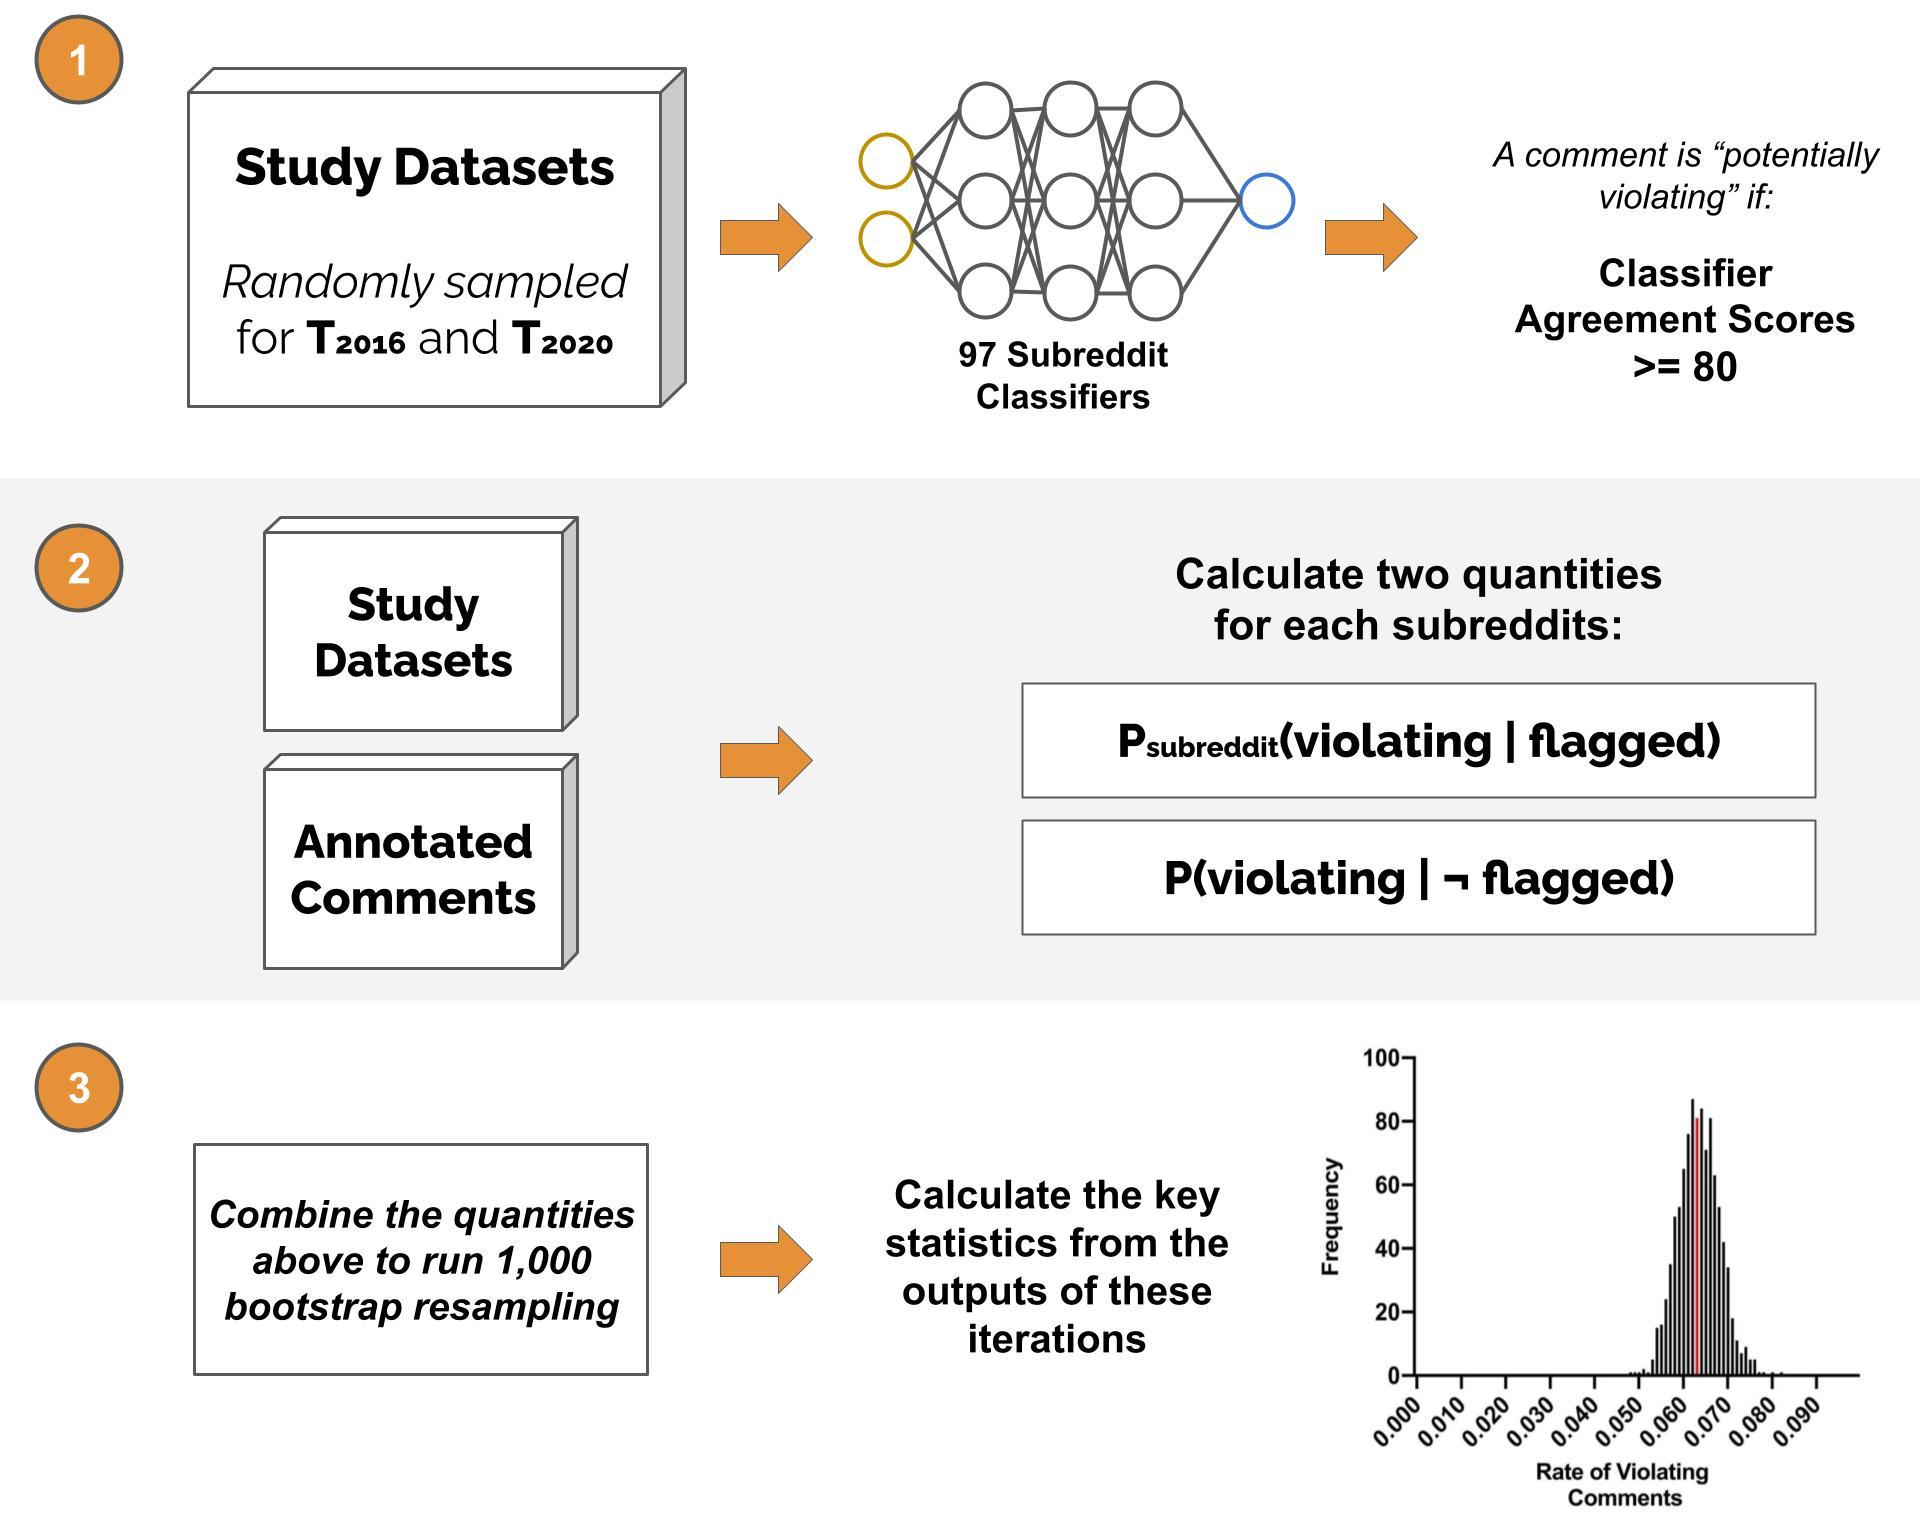
\includegraphics[width=1.0\textwidth]{content_minor_revision__Apr2022/images/bootstrap_workflow_6.jpg}
  \caption{\rnr{An overview of the sampling process in broad strokes. We start by randomly sampling unmoderated comments from $T_{2016}$ and $T_{2020}$ to generate our study datasets. We use these datasets and the annotated comments to calculate key quantities needed for our bootstrap resampling. We then combine these quantities to implement our resampling procedure, which we repeat 1,000 times for each time periods of our interest.}}
  \label{fig:bootstrap}
  \Description{Bootstrap resampling workflow}
\end{figure}


\subsection{\rnr{Bootstrapping Resampling Process}}
We took the following steps to sample our data for bootstrapping. For simplicity, we will describe our method with reference to the May 2016--March 2017 dataset, which we will refer to as $T_{2016}$. 

Intuitively, a bootstrap uses resampling with replacement to create a large number of parallel universes, each with the same number of comments as the original dataset, but each universe will have a slightly different number of norm violating comments due to the resampling with replacement. This variation across many parallel universes is what yields uncertainty confidence intervals on our estimates. However, each universe (bootstrap sample) must also contend with the fact that we have not manually annotated all 5 million comments in the dataset as violating or not. Rather than use a single fixed measurement of norm-violating comments per subreddit, which would ignore this source of uncertainty in the estimation, we resample our annotations over and over again with replacement to build in uncertainty due to our limited number of annotations. Figure~\ref{fig:bootstrap} provides an overview of this process, which is explained in detail below.

\subsubsection{\rnr{Study data and the flagged comments}} 
We began by randomly sampling a set of unmoderated comments. Specifically, we sampled 5,000 random comments from each of the study subreddits posted during this period dataset, for a total of 485,000 comments. These comments were sampled from the Pushshift Reddit corpus, which contains a complete capture of all comments on each subreddit. For clarity in presentation, we will call this sample of comments from 2016--2017, $T_{2016}$. We then ran all 97 subreddit classifiers on each of the sampled comments to calculate the classifier agreement score. Any comments that were flagged by at least 80 of the 97 classifiers as violating were labeled as \textit{flagged}.

\subsubsection{\rnr{Calculating intermediate probabilities}}
For the bootstrap, we needed to follow a procedure where we sample a comment, label it as flagged or not based on the classifiers, and then label flagged comments as violating or not based on human annotators. However, because we cannot tractably label every flagged comment in the bootstrap via human annotation, we relied on statistical generalization via the bootstrap. For this generalization to succeed, we require two empirically observed probabilities for each bootstrap iteration: $P_{subreddit}(violating \mid flagged)$, the true positive rate, the probability that a flagged comment in a particular subreddit is verified by annotators as an actual violation; $P(violating \mid \lnot flagged)$, the false negative rate, the probability that a comment that is not flagged as potentially violating via our classifiers is in fact violating according to our annotators.

\paragraph{$P_{subreddit}(violating \mid flagged)$.} The true positive rate, $P_{subreddit}(violating \mid flagged)$, carries uncertainty since we can only manually annotate a fixed number of comments per subreddit. To model this uncertainty, we re-estimate $P_{subreddit}(violating \mid flagged)$ with each bootstrap resample. Each iteration, for each subreddit, we take a random resample with replacement of the 32 flagged comments that annotators had labeled for each subreddit with each resample (e.g., sample 32 comments with replacement from the set of 32 flagged comments for the subreddit). This value of $P_{subreddit}(violating \mid flagged)$ is then used for that subreddit for that bootstrap iteration and varies with each iteration, capturing uncertainty in our estimate, and is used to help estimate whether a flagged comment in our sample is a true positive.

\paragraph{$P(violating \mid \lnot flagged)$.} Some comments that the classifiers do not believe to be macro norm violations will, in fact, be violations---and our bootstrap procedure must account for this so that it does not undercount the number of violations. To estimate the false negative rate, $P(violating \mid \lnot flagged)$, we use the sample of 1,000 \textit{non-flagged} unmoderated comments that we manually annotated in Section 3.4. These 1,000 comments showed a consistent 1\% false negative rate of our classifiers across 10 randomly chosen subreddits, so we treat this value as being consistent across all subreddits and do not parameterize it by subreddit. However, we still must model uncertainty in this estimate. So, for each bootstrap iteration, we resample 1,000 comments with replacement from the set of 1,000 comments and calculate $P(violating \mid \lnot flagged)$ as the proportion of comments that were not flagged as potentially violating but were in fact violating according to human annotators. We use this quantity to estimate whether a non-flagged comment in our sample is a false negative. As with the true positive rate, resampling with replacement will cause this value to vary from bootstrap iteration to iteration, critical to creating confidence intervals for our analysis.

\subsubsection{\rnr{Bootstrap resampling iteration procedure}}
These two probabilities enable our bootstrap procedure. In bootstrapping, we resample the dataset many times and measure the quantity of interest in each new instance. \rnr{In this study, we ran our bootstrapping procedure for 1,000 iterations (this is a typical number of iterations when conducting bootstrap resampling \cite{81_Bootstrap}). For each iteration, we resampled a number of comments that matched the complete number of comments on each of our study subreddits during our study period (i.e., 252,642,908 comments for $T_{2016}$). We also resample with replacement from the dataset of 5,000 classified comments each iteration, creating variation to model uncertainty in our sampling. Each bootstrap iteration also estimates new values for $P_{subreddit}(violating \mid flagged)$ and $P(violating \mid \lnot flagged)$ for each iteration, which combine to provide one datapoint in the final outcome distribution. In other words, each bootstrap sample creates an alternative universe of comments resampled from each subreddit, exhibiting natural variation in violation and moderation rates due to the random sampling.}

We illustrate this process with an example of bootstrap resampling the r/videos subreddit for $T_{2016}$. There were a total of 5,296,900 unmoderated comments that were on r/videos during $T_{2016}$. To populate each of these comments, we sampled a random comment from the subset of 5,000 random comments from r/videos that the classifiers had labeled. These 5,000 random comments had themselves been randomly sampled with replacement for this iteration of the bootstrap from the original set of 5,000 comments that were collected and classified. For r/videos, in one of the bootstrap samples, 1,249 of the 5,000 randomly sampled unmoderated comments (25\%) were flagged as potentially violating by the classifiers. If the sampled comment was flagged, then we randomly assign the comment as violating with probability $P_{r/videos}(violating \mid flagged)$ ($\approx 0.2$ in this bootstrap iteration) and attach the violation type(s) that human annotators tagged that comment with, and as not violating otherwise. If the sampled comment was not flagged, then we randomly assign the comment as violating with $P(violating \mid \lnot flagged)$ ($\approx 0.01$ in this iteration), and not violating otherwise. This process repeats to generate all 5,296,900 comments for r/videos.

We follow this process for all 97 subreddits, for all 1,000 bootstrap samples. The 1,000 samples provide a distribution and uncertainty estimate for the key statistics. Finally, through this process, we resample the same number of comments as the number of all unmoderated comments that were posted on these subreddits, some of which are labeled to be violating. So when we calculate the rate of unmoderated but violating comments in one bootstrap iteration, we add up the number of unmoderated but violating comments in each of the 97 subreddits and divide that by the number of all comments --- this gave us an estimation for r/videos, which was 5.95\% [2.16, 9.22] for $T_{2016}$, and 3.53\% [0.59, 9.14] for $T_{2020}$. This allows our bootstrap procedure to naturally take into account the different subreddit sizes --- through resampling more comments from the larger subreddits, the bootstrap will give more weight to the uncertainty on larger subreddits, in the analysis which are focused on the overall rates across the platform.

\subsubsection{2020 dataset}
As mentioned in the previous section, there are two periods of interest: one, from May 2016 to March 2017, the same period as when the moderated comments dataset $\mathcal{M}$ was collected, and the other from the last three weeks of December 2020, which we consider as a replication study on a slightly shorter but more recent timeframe. As we referred to the original dataset as $T_{2016}$, we will refer to the latter as $T_{2020}$. The process for $T_{2020}$ was identical to $T_{2016}$. Because $T_{2020}$ was a smaller dataset, however, its constituent samples were fewer in number. In particular, we \rnr{randomly} sampled 2,000 comments from each of the study subreddits instead of 5,000 commments, or fewer if the subreddit did not contain 2,000 comments during $T_{2020}$. This resulted in a total of 188,000 comments sampled and run through our 97 subreddit classifiers. Given the smaller sample size, the confidence intervals are wider for $T_{2020}$ than for $T_{2016}$.

\subsection{\rnr{Ablation Analysis with Fewer Annotations}}
Our bootstrap relies on a set of thousands of manually annotated comments from annotators. This gives rise to a possible threat to validity: that we did not manually annotate enough comments per subreddit to capture the uncertainty in the estimate per subreddit. To test whether this threat should be concerning, we performed an ablation analysis where we replicated our method using half of the manual annotations we had for each of the subreddits (that is, 16 annotations per subreddit instead of 32 for $T_{2016}$, and 4 per subreddit instead of 8 for $T_{2020}$). The main goal of this ablation analysis was to test how having fewer annotations impacts the uncertainty estimates of the bootstrap. Intuitively, as we have fewer and fewer samples, the confidence intervals will widen because if a rare event is sampled, it has a larger impact on the resulting estimate. We report our findings alongside our main results, in Section 6.
